\definecolor{Pianificate}{RGB}{51,102,204}
\definecolor{Consumate}{RGB}{32,18,77}

\pgfplotsset{
ybar, enlargelimits =0.10,
legend style ={at={(0.5,-0.5)},
anchor=north,
legend columns=-1},
ylabel={Ore},
xtick=data,
x tick label style={rotate=45,anchor=east},
symbolic x coords={Amministratore, Analista, Progettista, Programmatore, Responsabile, Verificatore},
}

\section{Preventivo a finire}
\label{consuntivo}

In questa sezione verrà presentato il preventivo a finire ovvero il preventivo al netto del consuntivo, sia per le ore che per i costi sostenuti. In base alle ore di differenza tra il preventivo e il consuntivo avremo che il bilancio è:
\begin{itemize}
\item \textbf{Positivo}, si sono risparmiate ore che potranno essere ricollocate in un periodo successivo;
\item \textbf{Negativo}, si sono consumate più ore di quante preventivate, per non fare deficit si dovranno rivedere le ore future;
\item \textbf{In pari}, sono state consumate esattamente le ore preventivate.
\end{itemize}

\subsection{Analisi}

In questo paragrafo viene riportato il consuntivo del periodo di \textit{Analisi}.

La tabella sottostante riporta le ore preventivate e le ore effettivamente impiegate (riportate tra parentesi) per ciascun componente del gruppo \GroupName{}.

\begin{table}[H]
\begin{tabular}{lccccccc}
\toprule
    \textbf{Nome}  & \multicolumn{6}{c}{\textbf{Ore per ruolo}} & \textbf{Ore totali} \\
     & Amm. & Ana. & Pgt. & Pgr. & Res. & Ver. & \\
    \midrule
    
    		Enrico Rotundo & 0 (+0) & 12 (-12) & 9 (-9) & 0 (+0) & 0 (+0) & 2 (-2) & 23 (-23) \\
	Federico Poli & 0 (+0) & 9 (-9) & 0 (+0) & 0 (+0) & 4 (-4) & 9 (-9) & 22 (-22) \\
	Giacomo Fornari & 9 (-9) & 2 (-2) & 0 (+0) & 0 (+0) & 5 (-5) & 4 (-4) & 20 (-20) \\
	Gianluca Donato & 0 (+0) & 10 (-10) & 0 (+0) & 0 (+0) & 0 (+0) & 11 (-11) & 21 (-21) \\
	Luca De Franceschi & 6 (-6) & 11 (-11) & 0 (+0) & 0 (+0) & 0 (+0) & 0 (+0) & 17 (-17) \\
	Nicolò Tresoldi & 15 (-15) & 0 (+0) & 0 (+0) & 0 (+0) & 5 (-5) & 0 (+0) & 20 (-20) \\
	Serena Girardi & 0 (+0) & 14 (-14) & 0 (+0) & 0 (+0) & 0 (+0) & 5 (-5) & 19 (-19) \\

    
    \bottomrule
\end{tabular}
\caption{Differenza preventivo consuntivo per componente, periodo di Analisi}
\end{table}

La tabella sottostante riporta le ore preventivate e le ore effettivamente impiegate (riportate tra parentesi) per ciascun ruolo presente nel periodo di \textit{Analisi}.

\begin{table}[H]
\begin{tabular}{lccccccc}
\toprule
    \textbf{Ruolo}  & \textbf{Ore} & \textbf{Costo} \\
    \midrule
    
    		Amministratore & 30 (+0) & 600 (+0) € \\
	Analista & 58 (-8) & 1450 (-200) € \\
	Progettista & 9 (-1) & 198 (-22) € \\
	Programmatore & 0 (+0) & 0 (+0) € \\
	Responsabile & 14 (+1) & 420 (+30) € \\
	Verificatore & 31 (+9) & 465 (+135) € \\
\hline
\textbf{Totale consuntivo} & +141 & +3190 € \\
\textbf{Totale preventivo} & +142 & +3133 € \\
\textbf{Differenza dei totali} & +1 & -57 € \\

    
    \bottomrule
\end{tabular}
\caption{Differenza preventivo consuntivo per ruolo, periodo di Analisi}
\end{table}

Viene di seguito incluso il grafico che illustra la differenza tra ore preventivate e ore effettivamente impiegate per ciascun ruolo nel periodo di \textit{Analisi}.

\begin{center}
\begin{figure}[H]
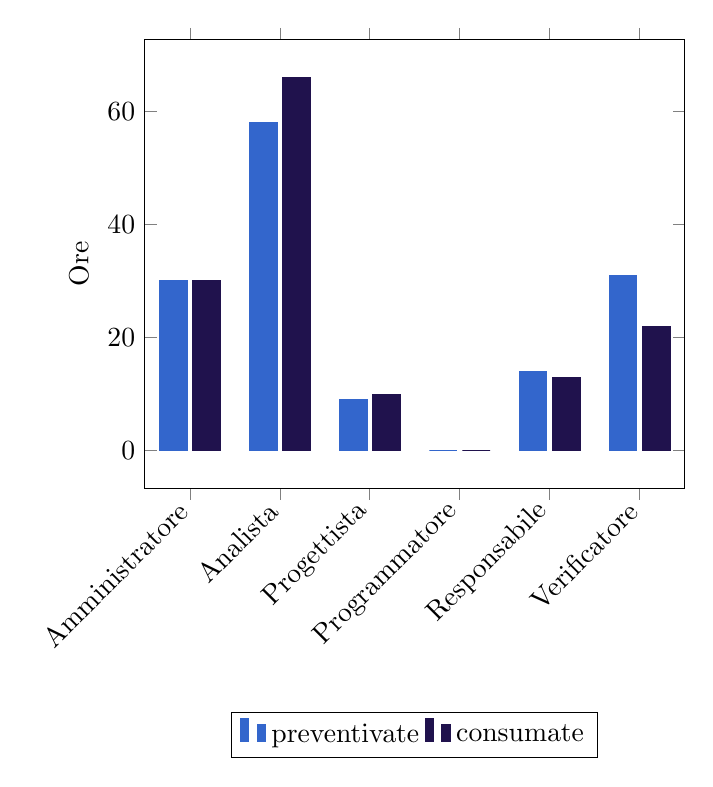
\begin{tikzpicture}
\begin{axis}
\addplot+[color=Pianificate] plotcoordinates {(Amministratore,30)(Analista,58)(Progettista,9)(Programmatore,0)(Responsabile,14)(Verificatore,31)};
\addplot+[color=Consumate] plotcoordinates {(Amministratore,30)(Analista,66)(Progettista,10)(Programmatore,0)(Responsabile,13)(Verificatore,22)};

\legend{preventivate,consumate}
\end{axis}
\end{tikzpicture}
\caption{Differenza preventivo consuntivo per ruolo, periodo di analisi}
\end{figure}
\end{center}

\subsection{Progettazione architetturale}

In questo paragrafo viene riportato il consuntivo del periodo di \textit{Progettazione architetturale}.

La tabella sottostante riporta le ore preventivate e le ore effettivamente impiegate (riportate tra parentesi) per ciascun componente del gruppo \GroupName{}.

\begin{table}[H]
\begin{tabular}{lccccccc}
\toprule
    \textbf{Nome}  & \multicolumn{6}{c}{\textbf{Ore per ruolo}} & \textbf{Ore totali} \\
     & Amm. & Ana. & Pgt. & Pgr. & Res. & Ver. & \\
    \midrule
    
    		Enrico Rotundo & 0 (+0) & 4 (+0) & 16 (+0) & 0 (+0) & 0 (+0) & 16 (+0) & 36 (+0) \\
	Federico Poli & 4 (+0) & 0 (+0) & 28 (+0) & 0 (+0) & 4 (+0) & 4 (+0) & 40 (+0) \\
	Giacomo Fornari & 8 (+0) & 2 (+0) & 8 (+0) & 0 (+0) & 4 (+0) & 22 (+0) & 44 (+0) \\
	Gianluca Donato & 6 (+0) & 8 (+0) & 14 (+0) & 0 (+0) & 4 (+0) & 8 (+0) & 40 (+0) \\
	Luca De Franceschi & 6 (+0) & 0 (+0) & 16 (+0) & 0 (+0) & 10 (+0) & 6 (+0) & 38 (+0) \\
	Nicolò Tresoldi & 10 (+0) & 0 (+0) & 8 (+0) & 0 (+0) & 4 (+3) & 8 (+0) & 30 (+3) \\
	Serena Girardi & 8 (+0) & 10 (+0) & 18 (+0) & 0 (+0) & 0 (+0) & 14 (+0) & 50 (+0) \\

    
    \bottomrule
\end{tabular}
\caption{Differenza preventivo consuntivo per componente, periodo di Progettazione Architetturale}
\end{table}

La tabella sottostante riporta le ore preventivate e le ore effettivamente impiegate (riportate tra parentesi) per ciascun ruolo presente nel periodo di \textit{Progettazione architetturale}.

\begin{table}[H]
\begin{tabular}{lccccccc}
\toprule
    \textbf{Ruolo}  & \textbf{Ore} & \textbf{Costo} \\
    \midrule
    
    		Amministratore & 42 (+0) & 840 (+0) € \\
	Analista & 24 (+0) & 600 (+0) € \\
	Progettista & 108 (+0) & 2376 (+0) € \\
	Programmatore & 0 (+0) & 0 (+0) € \\
	Responsabile & 26 (-3) & 780 (-90) € \\
	Verificatore & 78 (+0) & 1170 (+0) € \\
\hline
\textbf{Totale consuntivo} & +281 & +5856 € \\
\textbf{Totale preventivo} & +278 & +5766 € \\
\textbf{Differenza dei totali} & -3 & -90 € \\

    
    \bottomrule
\end{tabular}
\caption{Differenza preventivo consuntivo per ruolo, periodo di Progettazione Architetturale}
\end{table}

Viene di seguito incluso il grafico che illustra la differenza tra ore preventivate e ore effettivamente impiegate per ciascun ruolo nel periodo di \textit{Progettazione architetturale}.

\begin{center}
\begin{figure}[H]
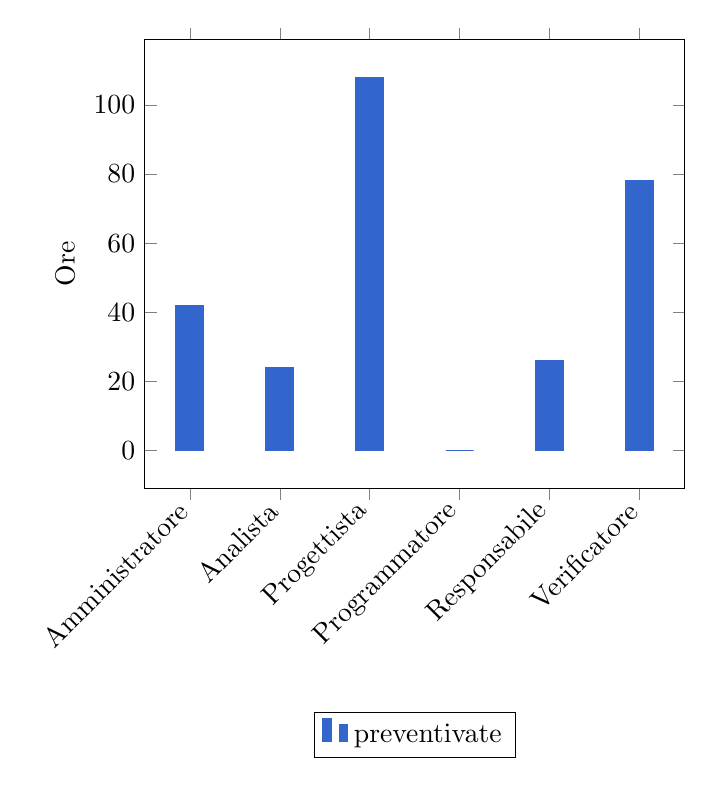
\begin{tikzpicture}
\begin{axis}
\addplot+[color=Pianificate] coordinates {(Amministratore,42)(Analista,24)(Progettista,108)(Programmatore,0)(Responsabile,26)(Verificatore,78)};

\legend{preventivate,consumate}
\end{axis}
\end{tikzpicture}
\caption{Differenza preventivo consuntivo per ruolo, periodo di progettazione architetturale}
\end{figure}
\end{center}

\subsection{Totale}

\begin{table}[H]
\begin{tabular}{lccccccc}
\toprule
    \textbf{Nome}  & \multicolumn{6}{c}{\textbf{Ore per ruolo}} & \textbf{Ore totali} \\
     & Amm. & Ana. & Pgt. & Pgr. & Res. & Ver. & \\
    \midrule
    
    		Enrico Rotundo & 0 (+0) & 16 (+2) & 25 (+1) & 0 (+0) & 0 (+0) & 18 (+0) & 59 (+3) \\
	Federico Poli & 4 (+0) & 9 (+2) & 28 (+2) & 0 (+0) & 8 (+3) & 13 (-4) & 62 (+3) \\
	Giacomo Fornari & 17 (+0) & 4 (+0) & 8 (+0) & 0 (+0) & 9 (+0) & 26 (+0) & 64 (+0) \\
	Gianluca Donato & 6 (+0) & 18 (+2) & 14 (+0) & 0 (+0) & 4 (+0) & 19 (-5) & 61 (-3) \\
	Luca De Franceschi & 12 (+0) & 11 (+2) & 16 (+0) & 0 (+0) & 6 (+0) & 10 (+0) & 55 (+2) \\
	Nicolò Tresoldi & 25 (+0) & 0 (+0) & 8 (+0) & 0 (+0) & 13 (+4) & 4 (+0) & 50 (+4) \\
	Serena Girardi & 8 (+0) & 24 (+0) & 18 (+0) & 0 (+0) & 0 (+0) & 19 (+0) & 69 (+0) \\

    
    \bottomrule
\end{tabular}

\caption{Ore per componente, periodo di Progettazione Architetturale}
\end{table}

\begin{table}[H]
\begin{tabular}{lccccccc}
\toprule
    \textbf{Ruolo}  & \textbf{Ore} & \textbf{Costo} \\
    \midrule
    
    		Amministratore & 72 (+0) & 1440 (+0) € \\
	Analista & 82 (-8) & 2050 (-200) € \\
	Progettista & 117 (-1) & 2574 (-22) € \\
	Programmatore & 0 (+0) & 0 (+0) € \\
	Responsabile & 40 (-5) & 1200 (-150) € \\
	Verificatore & 109 (+12) & 1635 (+172) € \\
\hline
\textbf{Totale consuntivo} & +423 & +9099 € \\
\textbf{Totale preventivo} & +420 & +8899 € \\
\textbf{Differenza dei totali} & -3 & -200 € \\

    
    \bottomrule
\end{tabular}
\caption{Ore per ruolo, periodo di Progettazione Architetturale}
\end{table}